\section{Sequence Diagram}

\begin{figure}[H]
	\makebox[\paperwidth][c]{
		\hspace*{-7.5cm}
		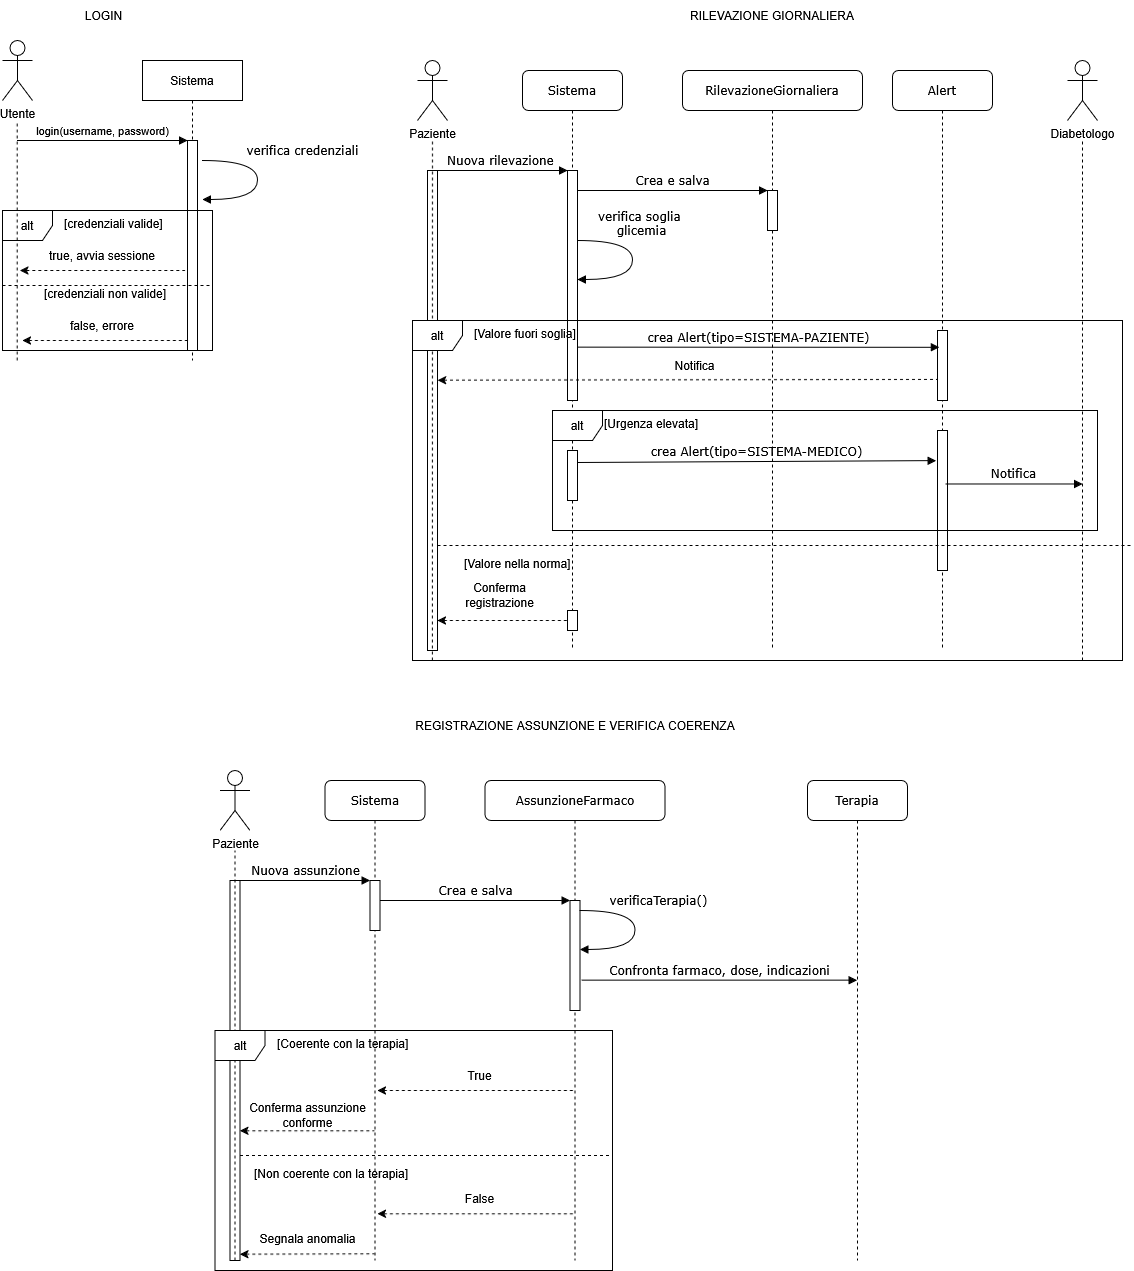
\includegraphics[
		height=0.92\textheight,
		keepaspectratio
		]{Immagini/SequenceDiagram11.png}
	}
	\caption{Sequence Diagram (Parte 1)}
	\label{fig:sequence-diagram_1}
\end{figure}

\begin{figure}[H]
	\makebox[\paperwidth][c]{
		\hspace*{-7.5cm}
		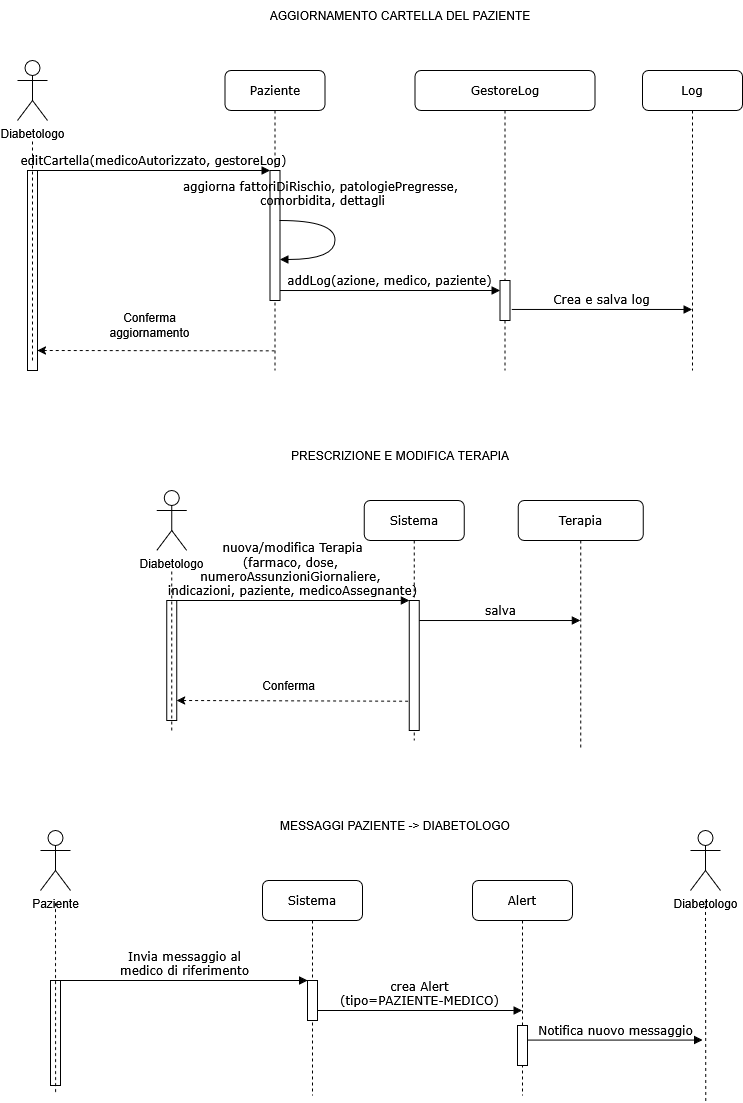
\includegraphics[
		width=0.98\paperwidth,
		height=0.98\textheight,
		keepaspectratio
		]{Immagini/SequenceDiagram33.png}
	}
	\caption{Sequence Diagram (Parte 2)}
	\label{fig:sequence-diagram_2}
\end{figure}

Login: L'utente inserisce username e password nella schermata di accesso. Il sistema inoltra le credenziali al database, il quale verifica la corrispondenza con un utente registrato. Se sono valide, viene avviata la sessione ed è aperta la schermata corrispondente al ruolo dell'utente. In caso contrario il sistema segnala un errore e  impedisce l'accesso.\\

Rilevazione giornaliera: il paziente inserisce i dati relativi a una nuova rilevazione, ovvero data, livello di glicemia, orario, orario dell'ultimo pasto e momento della rilevazione. Dopodiché il sistema la salva e verifica il livello di glicemia riportato rispetto alle soglie previste. Se esso è fuori dai limiti, viene creato un alert che notifica il diabetologo di riferimento di tale irregolarità, con un livello di urgenza maggiore se la glicemia si discosta particolarmente dalla norma. Il sistema conferma infine l'avvenuta  registrazione all'utente.\\

Registrazione di un'assunzione e verifica della coerenza: il paziente inserisce i dati relativi all'assunzione di un farmaco, indicando data, orario, quantità e terapia di riferimento. Tali dati vengono salvati e verificati, confrontandoli con le informazioni della terapia prescritta dal medico. Se essi sono discrepanti con la terapia, ciò viene segnalato all'utente.

Aggiornamento cartella del paziente: il diabetologo di riferimento accede alle informazioni del paziente e ne  modifica i dati, ovvero fattori di rischio, patologie pregresse, comorbidità e dettagli aggiuntivi. I dati vengono salvati e viene creato un log dell'operazione, associando la modifica all'utente che l'ha effettuata, in modo da mantenere la tracciabilità delle modifiche apportate.\\ 

Prescrizione e modifica di una terapia: il diabetologo di riferimento crea una nuova terapia oppure modifica le specifiche di una terapia già assegnata in passato modificando i dati rilevanti. Nel caso di modifica di una terapia condivisa da più pazienti, il sistema crea una nuova versione della terapia per il paziente interessato, evitando di modificare la terapia degli altri pazienti che continuano a utilizzare quella precedente.\\

Scambio di messaggi tra paziente e diabetologo: il paziente apre la schermata di comunicazione e scrive un messaggio al proprio medico di riferimento. Il medico viene notificato, può aprirlo e leggerlo.
 
 \section{Sequence Diagram del software progettato}
 
 \begin{figure}[H]
 	\centering
 	
 	\makebox[\paperwidth][c]{
 		\hspace*{-7.5cm}
 		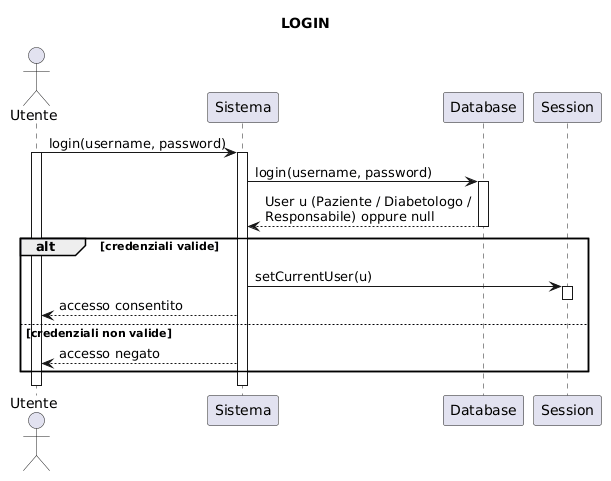
\includegraphics[
 		height=0.4\textheight,
 		keepaspectratio
 		]{Immagini/SequenceDiagramSW1.png}
 	}
 	
 	\vspace{0.1cm}
 	
 	\makebox[\paperwidth][c]{
 		\hspace*{-7.5cm}
 		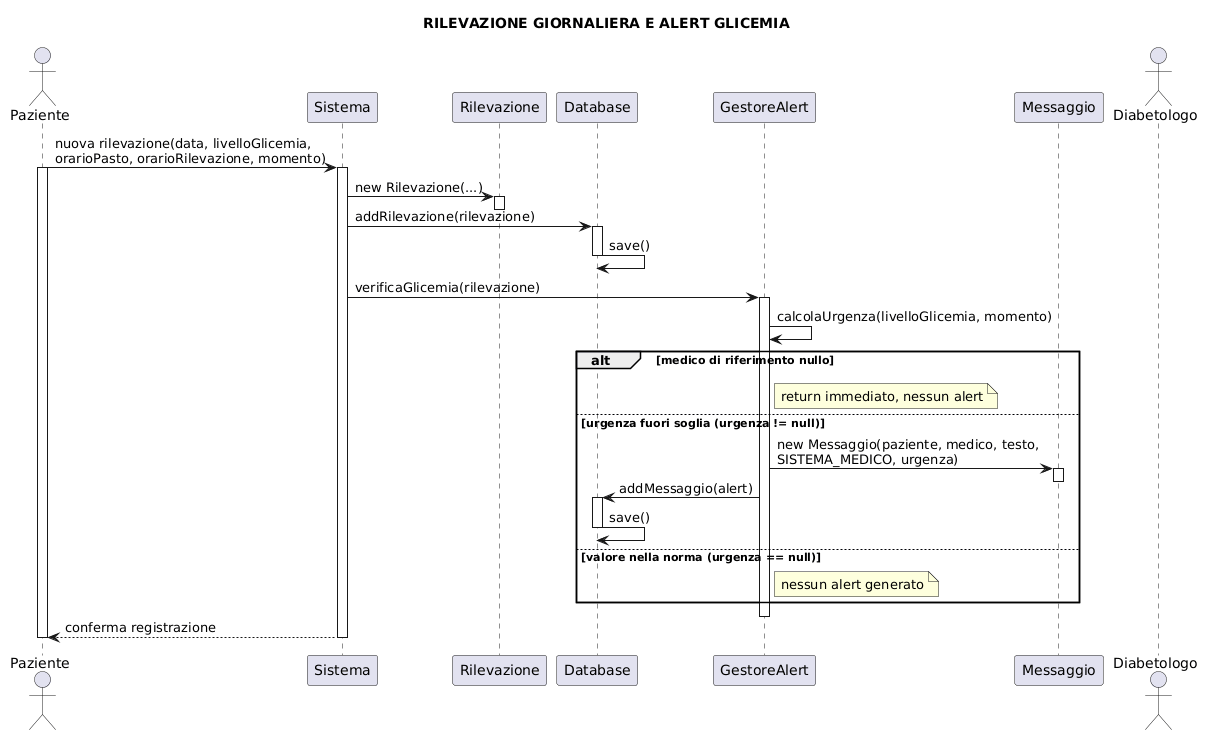
\includegraphics[
 		height=0.59\textheight,
 		keepaspectratio
 		]{Immagini/SequenceDiagramSW2.png}
 	}
 	
 	\label{fig:SD SF 1-2}
 \end{figure}
 
  \begin{figure}[H]
 	\centering
 	
 	\makebox[\paperwidth][c]{
 		\hspace*{-7.5cm}
 		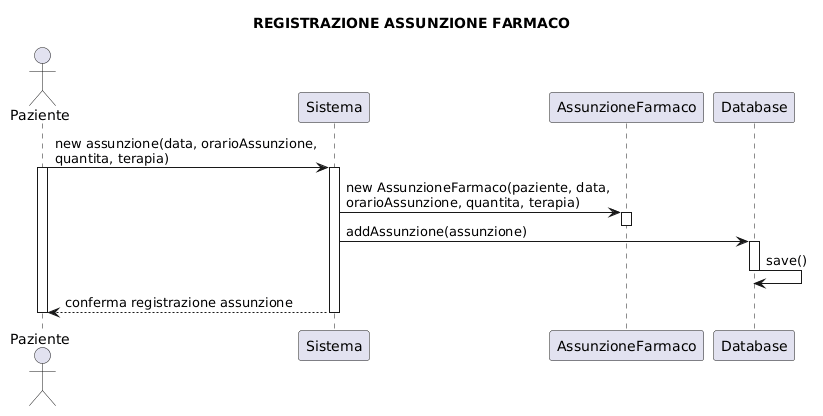
\includegraphics[
 		height=0.35\textheight,
 		keepaspectratio
 		]{Immagini/SequenceDiagramSW3.png}
 	}
 	
 	\vspace{0.1cm}
 	
 	\makebox[\paperwidth][c]{
 		\hspace*{-7.5cm}
 		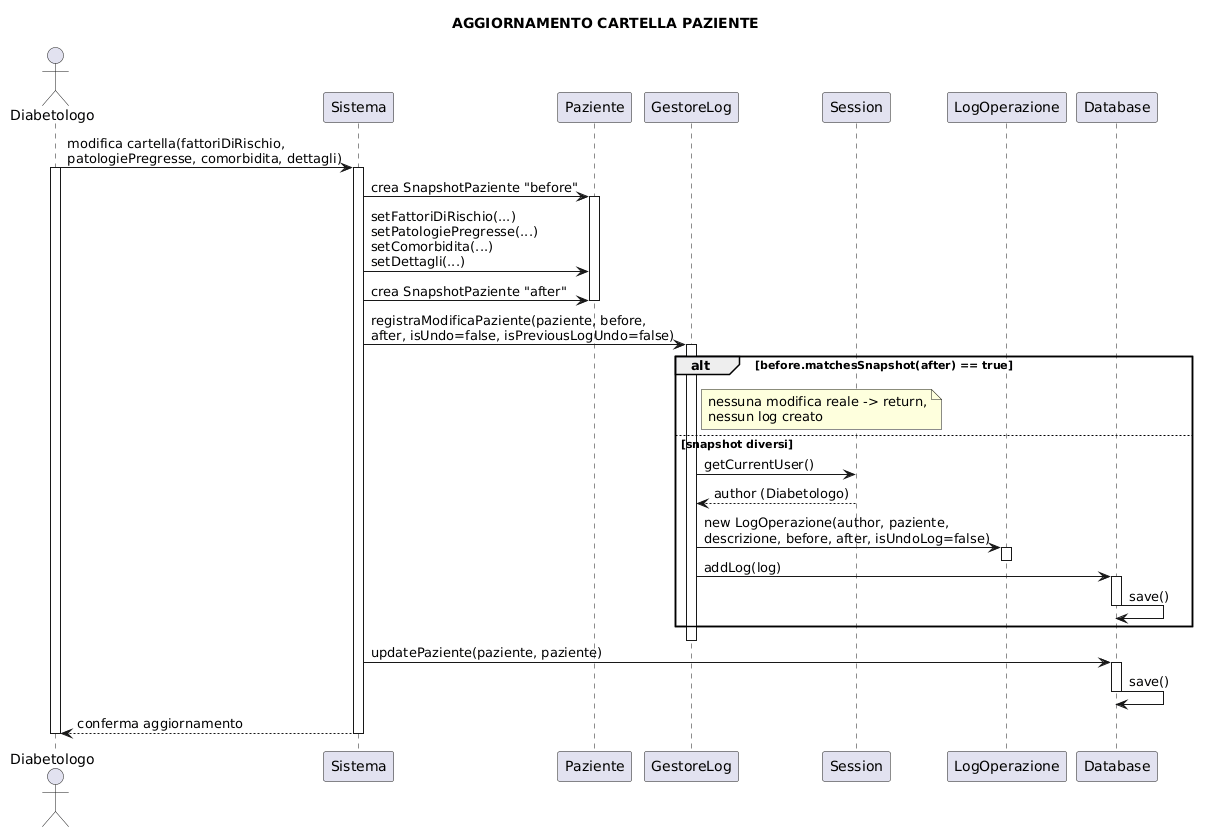
\includegraphics[
 		height=0.64\textheight,
 		keepaspectratio
 		]{Immagini/SequenceDiagramSW5.png}
 	}
 	
 	\label{fig:SD SF 3-5}
 \end{figure}
 
   \begin{figure}[H]
 	\centering
 	
 	\makebox[\paperwidth][c]{
 		\hspace*{-7.5cm}
 		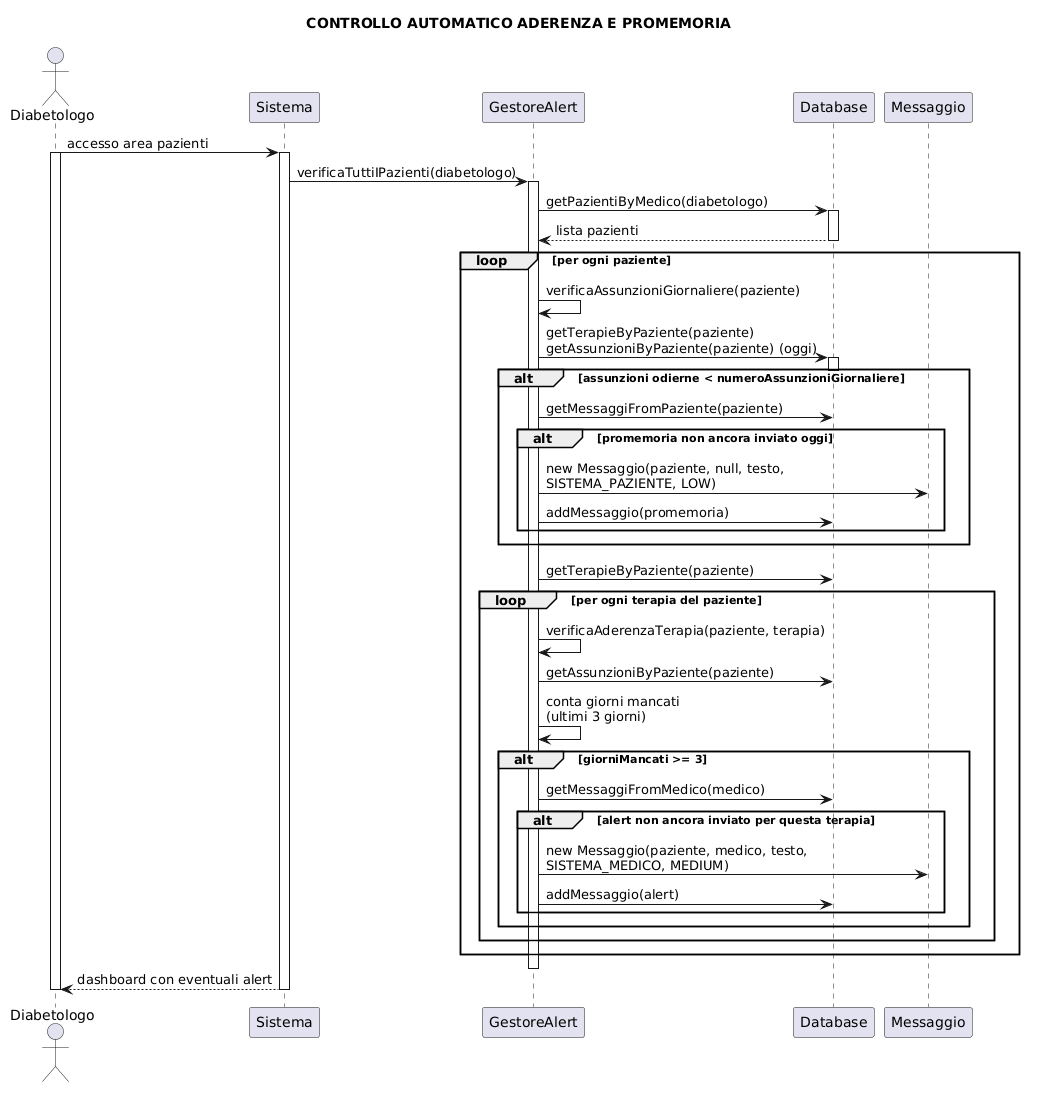
\includegraphics[
 		height=0.99\textheight,
 		keepaspectratio
 		]{Immagini/SequenceDiagramSW4.png}
 	}
 	 \label{fig:SD SF 4}

 \end{figure}
 
   \begin{figure}[H]
 	\centering
 	
 	\makebox[\paperwidth][c]{
 		\hspace*{-7.5cm}
 		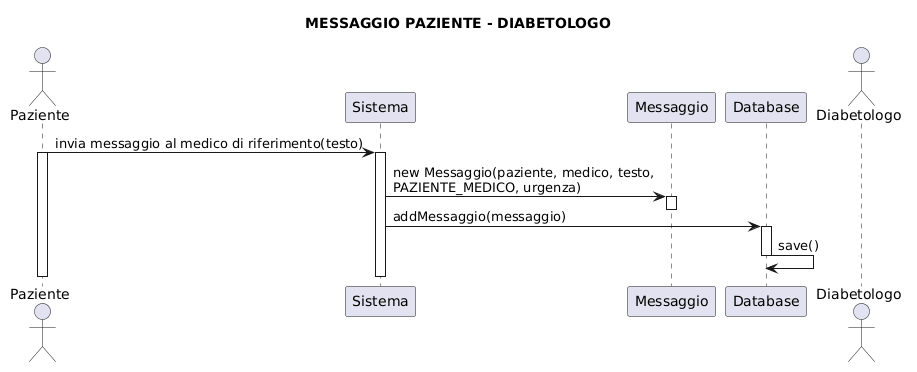
\includegraphics[
 		height=0.35\textheight,
 		keepaspectratio
 		]{Immagini/SequenceDiagramSW6.png}
 	}
 	
 	\vspace{0.1cm}
 	
 \makebox[\paperwidth][c]{
 	\hspace*{-7.5cm}
 	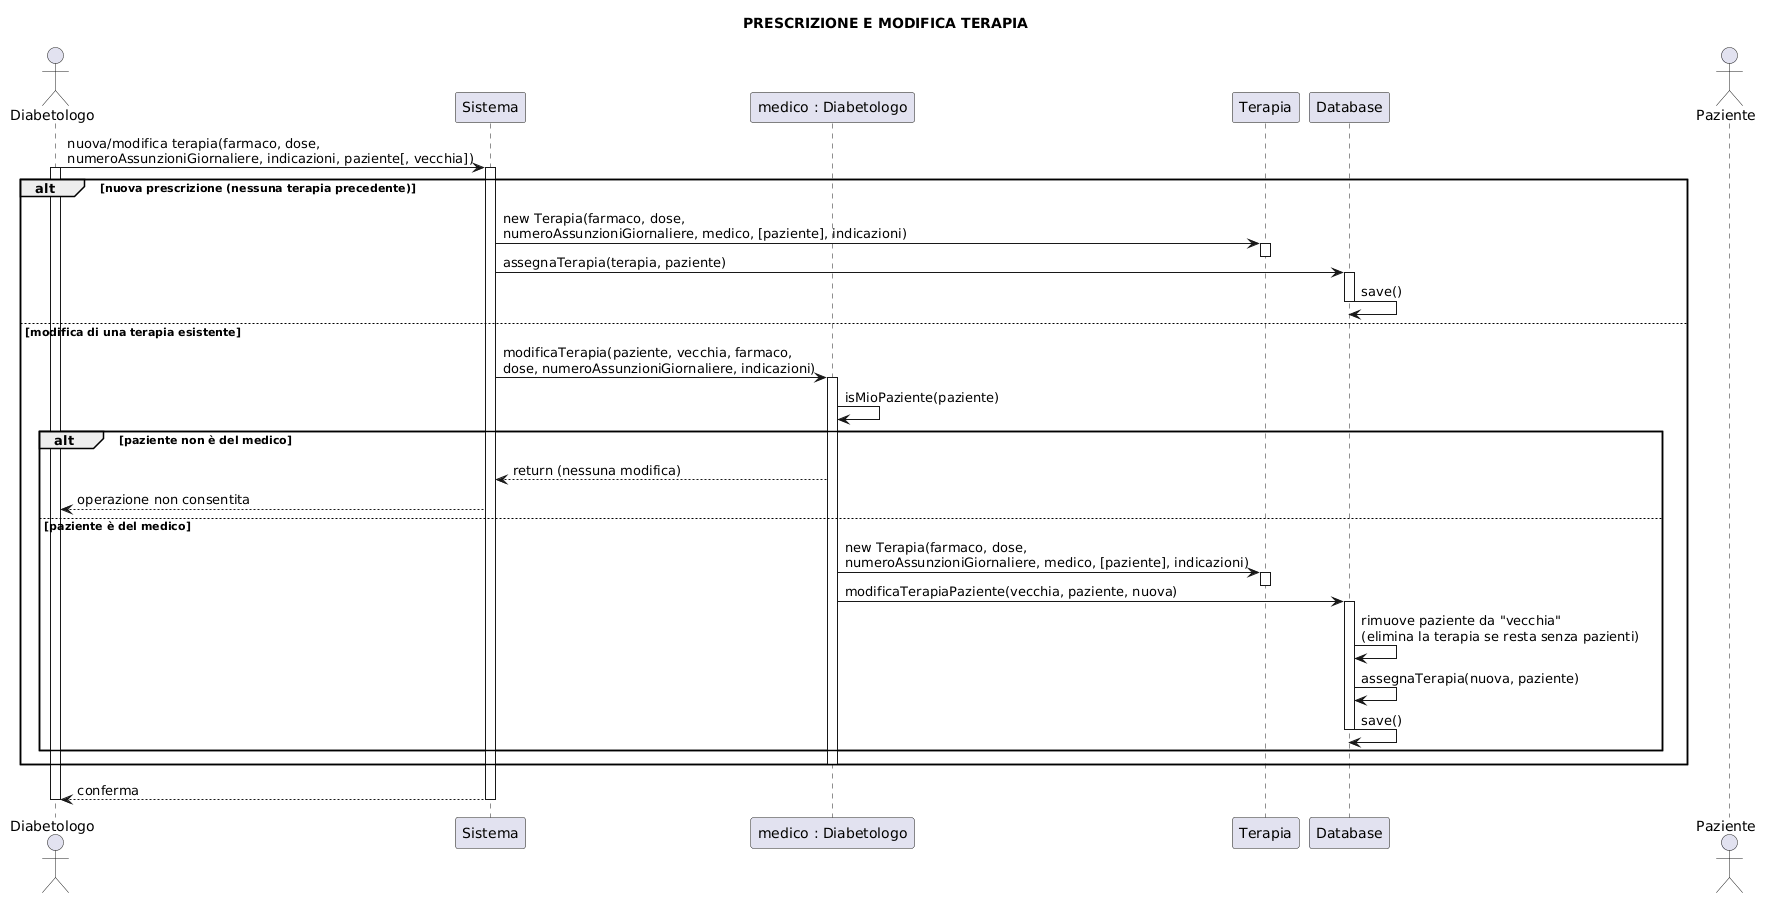
\includegraphics[
 	width=20cm,
 	height=0.7\textheight
 	]{Immagini/SequenceDiagramSW7.png}
 }
 	
 	\label{fig:SD SF 6-7}
 \end{figure}
 
Login: l'utente inserisce username e password nella schermata di accesso. Il sistema inoltra le credenziali al database, il quale verifica la corrispondenza con un utente registrato (Paziente, Diabetologo o Responsabile) oppure restituisce un valore nullo nel caso le credenziali non siano valide. Se sono valide, il sistema registra l'utente come corrente nella sessione attiva e consente l'accesso; in caso contrario, l'accesso viene negato.\\

Rilevazione giornaliera e alert glicemia: il paziente inserisce i dati di una nuova rilevazione (data, livello di glicemia, orario dell'ultimo pasto, orario della rilevazione e momento della giornata). Il sistema crea la rilevazione e la salva nel database, poi ne verifica il livello di glicemia rispetto alle soglie previste. Se il paziente non ha un medico di riferimento assegnato, il controllo termina senza generare alcun alert. Se invece il valore risulta fuori soglia, viene creato un messaggio di allerta destinato al medico, con un grado di urgenza calcolato in base a quanto il valore si discosta dalla norma, e il messaggio viene salvato nel database. Se il valore è nella norma, non viene generato alcun alert. In ogni caso, il sistema conferma al paziente l'avvenuta registrazione della rilevazione.\\

Registrazione assunzione farmaco: il paziente comunica al sistema l'avvenuta assunzione di un farmaco, specificando data, orario, quantità e terapia di riferimento. Il sistema crea l'oggetto assunzione e lo salva nel database, quindi conferma al paziente la registrazione avvenuta.\\

Controllo automatico aderenza e promemoria: quando il diabetologo accede all'area dei propri pazienti, il sistema avvia una verifica automatica su tutti i pazienti a lui assegnati. Per ciascun paziente, controlla innanzitutto se le assunzioni di farmaco registrate nella giornata sono inferiori al numero previsto dalla terapia: in tal caso, se non è già stato inviato un promemoria nella stessa giornata, ne viene generato uno a bassa urgenza destinato al paziente. Successivamente, per ogni terapia assegnata al paziente, il sistema conta i giorni mancati negli ultimi tre giorni; se le assunzioni mancate raggiungono o superano le tre e non è già stato inviato un alert per quella specifica terapia, viene generato un messaggio a urgenza media indirizzato al diabetologo. Al termine del controllo su tutti i pazienti, il sistema presenta al medico la dashboard con gli eventuali alert generati.\\

Aggiornamento cartella paziente: il diabetologo modifica i dati della cartella clinica del paziente (fattori di rischio, patologie pregresse, comorbidità e dettagli). Il sistema crea uno snapshot della cartella prima e dopo la modifica, per poterli confrontare. Se i due snapshot risultano identici, significa che non è stata apportata alcuna modifica reale e non viene creato alcun log. Se invece sono diversi, il sistema recupera l'utente corrente dalla sessione come autore dell'operazione, crea un log che registra la modifica (con i dati precedenti e modificati) e lo salva nel database. In entrambi i casi, la cartella del paziente viene infine aggiornata nel database e il sistema conferma l'operazione al diabetologo.\\

Messaggi paziente-diabetologo: il paziente invia un messaggio al proprio medico di riferimento tramite il sistema. Viene creato un nuovo messaggio, di tipo "paziente\_medico" e con il più basso livello di urgenza, che viene poi salvato nel database.\\

Prescrizione e modifica terapia: il diabetologo può assegnare a un paziente una nuova terapia oppure modificarne una già esistente, indicando farmaco, dose, numero di assunzioni giornaliere e indicazioni. Nel caso di una nuova prescrizione, ovvero non esiste nessuna terapia precedente, il sistema crea la terapia e la assegna direttamente al paziente, salvando il tutto nel database. Nel caso di modifica di una terapia esistente, il sistema verifica prima che il paziente sia effettivamente assegnato al medico: se non lo è, l'operazione viene negata. Se invece il paziente è del diabetologo, viene creata una nuova versione della terapia con i dati aggiornati; il paziente viene rimosso dalla terapia precedente (che viene eliminata se resta priva di pazienti) e associato alla nuova, così da non modificare la terapia degli altri pazienti che eventualmente la condividevano. Il sistema conferma infine l'operazione al diabetologo.\\


